% Version 2.20 of 2017/10/04
%
\documentclass[runningheads]{llncs}
%
\usepackage{graphicx}
% If you use the hyperref package, please uncomment the following line
% to display URLs in blue roman font according to Springer's eBook style:
% \renewcommand\UrlFont{\color{blue}\rmfamily}

\usepackage{orcidlink} % Orcid links
% Fix underscore in dois
\usepackage[strings]{underscore}

\begin{document}
%
\title{Instantaneous, understandable, and actionable soundness checking of industrial BPMN models}
%
%\titlerunning{Abbreviated paper title}
% If the paper title is too long for the running head, you can set
% an abbreviated paper title here
%
% \author{Tim Kr\"{a}uter\inst{1}\orcidlink{0000-0003-1795-0611} \and
% Adrian Rutle\inst{1}\orcidlink{0000-0002-4158-1644} \and
% Harald K\"{o}nig\inst{2,1}\orcidlink{0000-0001-6304-6311} \and
% Yngve Lamo\inst{1}\orcidlink{0000-0001-9196-1779}}
% %
% \authorrunning{T. Kräuter et al.}
% \institute{Western Norway University of Applied Sciences, Bergen, Norway 
% \email{tkra@hvl.no, aru@hvl.no, yla@hvl.no} \and
% University of Applied Sciences, FHDW, Hanover, Germany\\
% \email{harald.koenig@fhdw.de}}
%
\maketitle              % typeset the header of the contribution
%
\begin{abstract}
TODO
\keywords{
BPM \and
BPMN \and
BPMN analysis
}
\end{abstract}

% Up to 16 pages, including everything.

\section{Introduction}
% Why useful?
\cite{fahlandAnalysisDemandInstantaneous2011}
% Claims a lot of problems in workflow models, which can be found using soundness checks.
% Go over all three claims briefly: instantaneous (Definition), understandable (soundness properties are hard to understand for modelers), and actionable (comparable to quick fixes).

% Understandable/Visualization is missing in the figure: instantaneous and actionable are there.
\begin{figure}[ht]
	\centering
	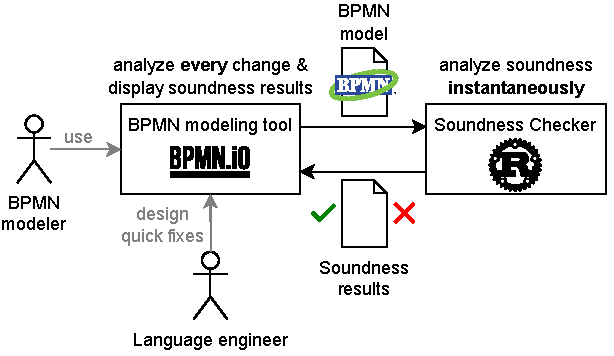
\includegraphics[width=1\textwidth]{images/overview}
	\caption{Overview of the approach}
	\label{fig:overview}
\end{figure}

% Soundness stuff taken from which adopted it for BPMN
\cite{corradiniClassificationBPMNCollaborations2018}

% One example should be introduced here, which then is picked up throughout the paper.
% Wrong gateway usage?
% Instantaneous: The model checks in 500ms or less.
% Understandable: Highlight problematic elements + show the visualization of a counterexample using that model.
% Actionable: Provide quick fixes that resolve soundness violation --> check if changes fix the property before showing it to the user.

\section{Instantaneous}
Instantaneous definition from here: \cite{fahlandAnalysisDemandInstantaneous2011}
500ms or less

% Provide empirical evidence that it is instantaneous. Use repositories and synthetic benchmarks with increasing model size and degree of parallelity. --> Maybe in a independent section and link to the results here
% Add all those datasets with artifacts using a Zenodo link --> Artifacts badge

These guys have some benchmarks:
\cite{corradiniFormalApproachAnalysis2021}

\section{Understandable}

% Highlight directly and instantly in the diagram --> Overlays (and colors)
% Interactive visualization of counterexamples.
\cite{camundaservicesgmbhBpmnjsTokenSimulation2024}

\section{Actionable}

% Quick fix providers/analysis resolvers/solution strategies/resolution strategies coded for the different soundness properties.
% Custom quick fix providers are also possible in the future with access to model-checking

When possible, we detect errors in the BPMN model and provide an automatic fix similar to quick fixes in IDEs.
Modelers can then select these quick fixes to resolve a specific soundness property.

Since checking soundness is inexpensive, the user can apply the quick fix and instantly get feedback on the changes.
If he is unhappy with the result, a user can undo these changes immediately since each quick fix is a \textit{command} (see command pattern \cite{gammaDesignPatternsElements1995}).
A user might not like a quick fix if it not only fixes a specific property but also has unintended side effects.
For example, it might invalidate a different soundness property.

In the following sections, we describe the implemented resolution strategies for the different soundness properties in detail.
However, we do not expect these strategies to cover all possible resolutions and fit all applications.
Thus, our framework is extensible, so other developers can provide additional or custom resolution strategies (dependency injection, decoupled analysis from handling from showing the errors).
% --> Add before and after figures for each maybe and link to the example demo page hosted somewhere (azure).

\subsection{Safeness}
1. Change gateways to match if gateways are the problem.

2. Add a parallel gateway if an implicit exclusive gateway is encoded (highlight command undoes all the changes in one).

3. Add an exclusive gateway if an implicit parallel gateway is encoded (command undo).
\subsection{Proper Completion}
1. If multiple incoming sequence flows are the cause, we can add a unique end event for each other than the first sf (highlight undo all the changes)

2. If only one sequence flow but the end event is "unproper" this is due to no safeness.
\subsection{Option to Complete}
Analyze the counter-example provided by Rust and try to locate where tokens are stuck (token locations + pg + multiple incoming flows).
% --> Could also be due to untriggered events --> future work.

\subsubsection{Resolution} \textbf{(1)} Change the pg to an exclusive gateway.

\textbf{(2)} Try to find the exclusive split and make that parallel. 
\subsection{No Dead Activities}
A dead activity might have multiple reasons:
\textbf{(1)} The simplest reason is that the activity is disconnected, i.e., it has no incoming sequence flow.
Disconnected activities must not be dead, but they violate best practices and are warned against by BPMN linters such as \cite[rule no-disconnected]{camundaservicesgmbhBpmnlint2024}.
\textbf{(2)} An activity can also be part of the BPMN model that is not reachable during execution, for example, because a parallel gateway preceding the activity cannot be executed.
% Could also be behind events that are never triggered.

\subsubsection{Resolution}
If the activity is disconnected \textbf{(1)}, we can propose connecting it to the nearest flow node.
However, this flow node should not be disconnected from itself.
Concretely, we assume modeling from left to right, such as all the other automatic layout mechanisms in bpmn-js \cite{camundaservicesgmbhBpmnjs2024} to find the leftmost nearest flow-node to connect.
\autoref{fig:noDeadActivitiesQuickFix} shows an example where this quick fix is applied.
As in the other examples, new elements are colored in green.

\begin{figure}[ht]
	\centering
	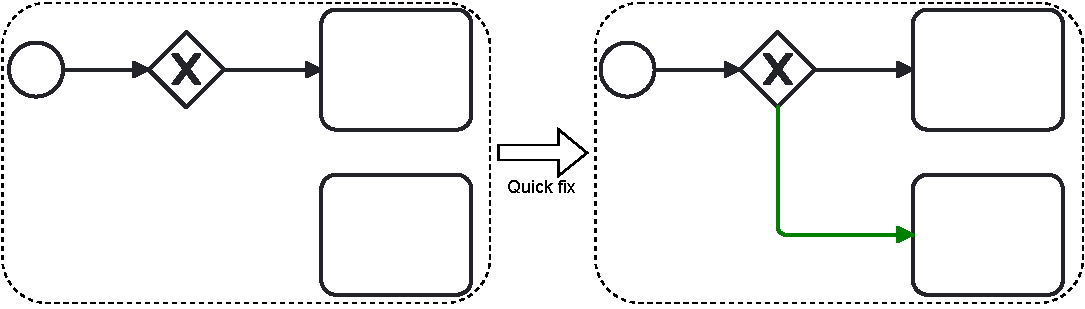
\includegraphics[width=1\textwidth]{images/dead}
	\caption{Quick fix connecting a disconnected activity}
	\label{fig:noDeadActivitiesQuickFix}
\end{figure}

In case \textbf{(2)} when the dead activity is connected, this will often lead to processes that cannot terminate, i.e., violate \textit{Option to Complete}.
Thus, other quick fixes for Option to complete can apply, which will also resolve dead activities.

\section{Implementation}

\subsection{Rust}
% Why in Rust?
% Low-level language with modern features.
% Highlight Rusts speed and safety claims
% Good for CLI tools such as this
% Zero-copy?
% Zero-overhead abstractions --> related to speed
% Reimplement in rust meme

\subsection{BPMN semantics}
% Describe the runtime model. What is a state? --> Draw a UML diagram
% Describe what the initial state is. --> Could be configurable in the future.
% Describe BPMN semantics with some diagrams for some examples.
% Use a good running example with a modeling error that wasn't used before (double-blind).

\subsection{Description}
% Tool UI with screenshot
\cite{camundaservicesgmbhBpmnjs2024}
% Tool architecture? UI in JS and backend in Rust.
% Just the model checker as a CLI app or a CLI that starts the whole thing as a service.


\section{Scalability analysis}

\subsection{Growing model size}
% Cite my LMCS paper here if already published.
% Briefly recap the method, but we only test in steps of 10.
% Should include those models somewhere

\subsection{Growing degrees of parallelism}
% Cite the other paper here with parallelism

\subsection{Industrial models}
% Check that we can check and analyze models from these model repositories cited anywhere.

\section{Related work}

% Different ways of comparison
% 1. BPMN features supported (sub of 2.)
% 2. Capabilities (Which soundness properties are supported, custom properties, counter-example visualization, tool maturity, tool integration, actionability of the tool, etc.)
% 3. Performance using different benchmarks. --> Needs its own paper where everyone can contribute.

\cite{krauterFormalizationAnalysisBPMN2023} % Also add LMCS citation here.

\cite{vangorpVisualTokenbasedFormalization2013}

\cite{corradiniBProVeToolSupport2017,corradiniFormalApproachAnalysis2021}

\section{Limitations \& Threats to Validity}

\section{Conclusion \& Future work}

\bibliographystyle{splncs04} 
\bibliography{bib}

\end{document}
